\documentclass{article}
\usepackage[T1]{fontenc}
\usepackage{lmodern}
\usepackage{graphicx}
\usepackage{amsmath,amssymb}
\usepackage[a4paper,margin=2cm]{geometry}
\usepackage[absolute,overlay]{textpos}
\setlength{\TPHorizModule}{1mm}
\setlength{\TPVertModule}{1mm}
\usepackage[indonesian]{babel}
\usepackage{hyperref}
\setlength{\emergencystretch}{2em}
% unit: Halaman 56

\begin{document}

% === Halaman 56 (python/native) ===

56

Queen Mary

◼Pada Abad ke-17, sejarah kriptografi 

pernah mencatat korban di Inggris.

◼Queen Mary of Scotland,  dipancung 

setelah pesan rahasianya dari balik penjara 

(sebuah cipherteks yang isinya rencana 

membunuh Ratu Elizabeth I) pada Abad 

Pertengahan berhasil dipecahkan oleh 

Thomas Phelippes, seorang pemecah kode 

(codebreaker).

% deskripsi: gambar native xref 270
\noindent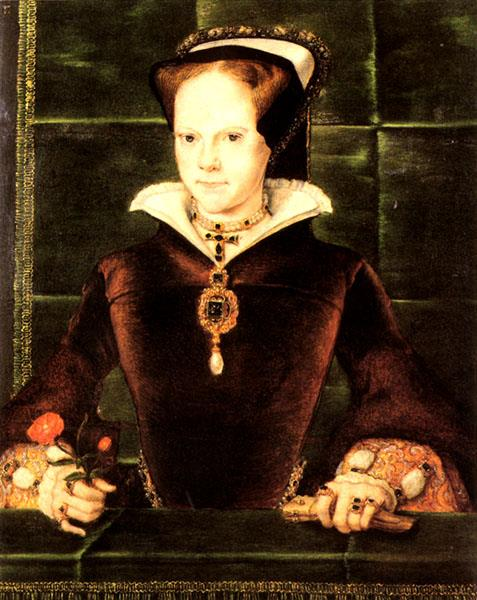
\includegraphics[width=0.85\textwidth]{../../images/python/page_056_img_01.jpeg}

\end{document}
